\section{电学}

\subsection{静电场}

\begin{formulatab}{静电场}
  \multicolumn{2}{l}{\textbf{基本定义与等式}}\\
  场强定义&$E=\frac{F}{q}$\\
  电势定义&$\varphi = \frac{W}{q}$\\
  电势差定义&$U_{AB}=\varphi_A-\varphi_B$\\
  电场力做功&$W=qU_{AB}=W_A-W_B=\sum qE\Delta d$\\
  \multicolumn{2}{l}{\textbf{匀强电场规律}}\\
  电势差与场强关系&$U=Ed$\\
  \multicolumn{2}{l}{\textbf{点电荷}}\\
  库仑定律&$F=\frac{kQq}{r^2}$\\
  点电荷电场强度&$E=\frac{kQ}{r^2}$\\
  点电荷电势&$\varphi=\frac{kQ}{r}$\\
  点电荷电势能&$W=\frac{kQq}{r}$\\
  \multicolumn{2}{l}{\textbf{连续分布电荷}}\\
  无限长直导线电场强度&$E=\frac{2k\lambda}{r}$\\
  无限大平面电场强度&$E=2\pi k\sigma$\\
  环形带电体轴线上电场强度&$E=\frac{kQL}{(L^2+R^2)^{3/2}}$\\
  环形带电体轴线上电势&$\varphi=\frac{kQ}{\sqrt{L^2+R^2}}$\\
  球形带电体外电场强度&$E=\frac{kQ}{r^2}$\\
  球形带电体外电势&$\varphi=\frac{kQ}{r}$\\
  球形带电体内电场强度&$E=0$\\
  球形带电体内电势&$\varphi=\frac{kQ}{R}$\\
  \multicolumn{2}{l}{\textbf{电容器}}\\
  电容决定式&$C=\varepsilon_0 \varepsilon_r \frac{S}{d}$\\
  真空介电常数关系&$k = \frac{1}{4\pi \varepsilon_0}$\\
  电容器能量&$E = \frac{1}{2} C U^2 = \frac{1}{2}\frac{Q^2}{C} = \frac{Q U}{2}$\\
  \multicolumn{2}{l}{\textbf{电场中的运动}}\\
  加速电场动能&$qU=\frac{1}{2}mv^2,\quad v=\sqrt{\frac{2qU}{m}}$\\
  加速电场动量&$qU=\frac{p^2}{2m},\quad p=\sqrt{2mqU}$\\
  竖直加速度&$a_y=\frac{qU}{md}$\\
  竖直速度&$v_y=a_yt=\frac{2y}{t}$\\
  竖直偏移量&$y=\frac{1}{2}a_yt^2$\\
  平抛推论&$\tan\theta=\frac{v_0}{v_y}=\frac{2y}{x}$\\
\end{formulatab}

其中 $C$ 为电容，$\varepsilon_0$ 为真空介电常数，$\varepsilon_r$ 为介质的相对介电常数，$S$ 为极板面积，$d$ 为极板间距离。

\textbf{电容器描述：}
电容器存储电能的元件，由两个导体之间隔着绝缘材料构成。平行板电容器是由两块平行放置的导体板组成，中间夹有绝缘介质。常用于研究电容器的基本性质。

\textbf{电容器充放电：}
电容器的充电过程是指在外加电压作用下，电容器两极板之间积累电荷的过程；放电过程是指电容器释放储存的电能，电荷流向外部电路的过程。只有在电容器两极板间存在电势差（即外加电源或电压）时，电容器才能充电。充电过程中，电流方向为正极板流入、负极板流出，直到两极板间的电势差等于外加电压时，充电过程结束，电流为零。

\textbf{充电过程中电流和电压的变化：}
电容器刚开始充电时，极板间电压为零，电流最大；随着充电进行，极板间电压逐渐升高，电流逐渐减小；当极板间电压等于外加电压时，电流减小到零，充电过程结束。

电容器存在击穿电压，当电压过大时电容器中间的绝缘材料就会被击穿，使得电容器被破坏。

\noindent\textbf{电容器注意事项：}
\begin{itemize}
  \item 电容器可以进行串并联，并联电容器，等效电容为电容器电容之和，串联电容器，等效电容规律和并联电阻相同。
\end{itemize}

\noindent\textbf{静电场注意事项：}
\begin{itemize}
  \item $\lambda$为线电荷密度，$\sigma$为面电荷密度，$R$为球体半径，$L$为轴线上距离球心的距离
  \item 电场力做功只与电荷初末位置有关，与路径无关
  \item 电势能增加，一般情况下，机械能减少
  \item 电场力做功时需要进行投影：$W=qEd\cos\theta$
  \item 电场线与等势面垂直
  \item 在匀强电场中，两点所在直线的场强均匀，可以通过$E'=\frac{U}{d}$求出
  \item 固定水平位移时，合速度最小时，水平与竖直方向速度相等
\end{itemize}

\subsection{电路}

\begin{formulatab}{电路}
  \multicolumn{2}{l}{\textbf{电流}}\\
  电流定义式&$I=\frac{Q}{t}$\\
  电流决定式&$I = nqSv$\\
  \multicolumn{2}{l}{\textbf{电阻}}\\
  电阻定义式&$R=\frac{U}{I}$\\
  电阻决定式&$R=\rho\frac{l}{S}$\\
  \multicolumn{2}{l}{\textbf{电容}}\\
  电容定义式&$C=\frac{Q}{U}$\\
  电容决定式&$C=\frac{\epsilon S}{4\pi kd}$\\
  电容器能量&$W=\frac{1}{2} CU^2=\frac{Q^2}{2C}=\frac{1}{2} QU$\\
  \multicolumn{2}{l}{\textbf{电源}}\\
  电动势&$E=\frac{W_{\text{非静电力}}}{q}$\\
  \multicolumn{2}{l}{\textbf{闭合电路欧姆定律}}\\
  含有外电阻和内阻&$E=I(R+r)$\\
  不含外电路电压（纯电阻）&$U=IR$\\
  不含外电阻&$U=E-Ir$\\
  不含电流（纯电源）&$U=E\frac{R}{R+r}$\\
  \multicolumn{2}{l}{\textbf{电阻的连接}}\\
  串联规律&$R=R_1+R_2+\cdots R_n$\\
  并联规律&$\frac{1}{R}=\frac{1}{R_1}+\frac{1}{R_2}+\cdots \frac{1}{R_n}$\\
  \multicolumn{2}{l}{\textbf{电表改装}}\\
  电流表简易改装（分流）&$R=\frac{I_gR_g}{I_{\text{量程}}-I_g}\approx \frac{I_gR_g}{I_{\text{量程}}}$\\
  电压表简易改装（增压）&$R=\frac{U_{\text{量程}}}{I_g}-R_g$\\
  欧姆表改装&$E=i(r+R_g+R_{\Omega}+R_x)$\\
  $R_x$表达式&$R_x=\frac{E}{i}-\frac{E}{I_g}=E\frac{I_g-i}{iI_g}$\\
  欧姆表中值电阻&$R_{\text{中值电阻}}=\frac{E}{I_g}=R_{\text{内}}$\\
  \multicolumn{2}{l}{\textbf{电流表改装的线性关系}}\\
  \multicolumn{2}{l}{\textbf{电功率}}\\
  电功率定义式&$P=UI$\\
  纯电阻功率&$P=P_{\text{热}}=I^2R=\frac{U^2}{R}$\\
  非纯电阻总功率&$P=UI$\\
  非纯电阻热功率&$P=I^2R$\\
  非纯电阻输出功率&$P=UI-I^2R$\\
  电源总功率&$P=EI=\frac{E^2}{R+r}\le \frac{E^2}{r}$\\
  电源热功率&$P=I^2r=\left(\frac{E}{R+r}\right)^2r\le \frac{E^2}{r}$\\
  电源输出功率&$P=UI=(E-Ir)I=\left(\frac{E}{r}-I\right)Ir\le \frac{E^2}{4r}$\\
  含纯电阻的输出功率&$P=\left(\frac{E}{R+r}\right)^2R=\frac{E^2}{R+\frac{r^2}{R}+2r}\le \frac{E^2}{4r}$\\
  电源效率&$\eta=\frac{P_{\text{输出}}}{P_{\text{总}}}=\frac{U}{E}=\frac{R}{R+r}$\\
  \multicolumn{2}{l}{\textbf{电桥测电阻}}\\
  电桥平衡条件&$R_x=\frac{R_2}{R_1}R_{\Omega}=\frac{l_L}{l_R}R_\Omega$\\
\end{formulatab}

表头电流与被测电阻成反比，表盘才会不均匀。

\textbf{游标卡尺和螺旋测微器使用}
\begin{center}
  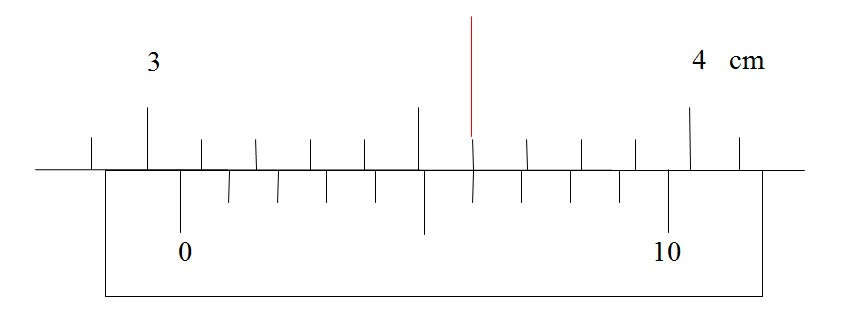
\includegraphics[width=0.6\columnwidth]{../assets/游标卡尺读数.jpg}
\end{center}
\textbf{游标卡尺读数方法：}\\
有两种方法读游标卡尺读数，\\
\textbf{方法一}：下方副尺0刻度线所在位置主尺的读数记为$N$（上图应该是3cm处，但是不到31mm）\\
然后找到副尺上与主尺刻度线对齐的刻度线的小格数，记为$m$，\\
游标卡尺读数$=N+m\times \text{游标卡尺精度}$mm\\
如上，为$ 30+6\times 0.1 \text{mm} = 30.6\text{mm}$\\
\textbf{方法二}：找到主尺与副尺刻度线\textbf{对齐}所在位置的读数，记为$N$，\\
找到副尺上与主尺刻度线\textbf{对齐}的刻度线对应的小格数，记为$m$，\\
游标卡尺读数为$=N-\frac{\text{副尺总长度}}{\text{副尺总格子数}}\times m$mm\\
如上，为$ 36 - \frac{6}{10}\times 9 \text{mm} = 30.6\text{mm}$\\
\begin{center}
  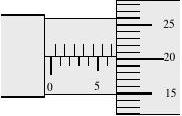
\includegraphics[width=0.6\columnwidth]{../assets/螺旋测微器读数.jpg}
\end{center}
\textbf{螺旋测微器读数方法：}\\
先确定右侧旋转筒左侧线所指的主尺半格数，注意上面也有一排刻度线，当超过主尺刻度线时，主尺读数需要加0.5mm，\\
然后读取右侧旋转筒上与主尺左侧线对齐的刻度线数，乘以螺旋测微器的精度0.01mm，注意需要估读一位，尽量估读准确一点。\\
最后螺旋测微器读数$=$主尺读数$+$旋转筒读数。\\
如上，为$ 6.5 \text{mm} + 20.3\times 0.01 \text{mm} = 6.703\text{mm}$

\noindent\textbf{电路中的基本认识：}
\begin{itemize}
  \item 恒压源的正极电势恒定比负极大$E$
  \item 恒流源干路电流恒定为$I$
  \item 沿电流方向电势降低
  \item 电势降低量$U=RI$
  \item 对电路中任意节点：$\sum I_{in}=\sum I_{out}$
  \item 导线的内阻为0，所以导线可以任意长度变化
  \item 理想电流表视为导线，理想电压表视为断路
  \item 电容器充满电或稳定状态都视为断路
  \item 电容器充电过程视为电阻
  \item 电容器放电视为理想电源
  \item 断路应该被视为是一个无穷大的电阻接在断路的导线两端
  \item 任何部分电阻增大都会导致总电阻增大，反之亦然
\end{itemize}

\textbf{电源功率图像：}
{
  \centering
  \textbf{电源总功率与电流图像}\\
  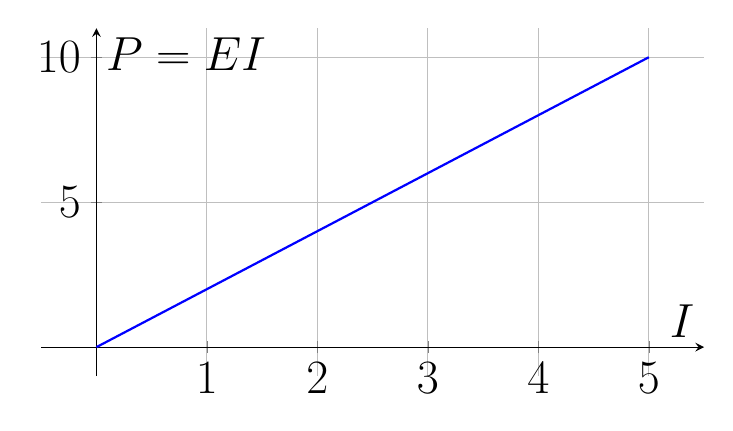
\begin{tikzpicture}
    \begin{axis}[
        width=10cm, height=6cm,
        axis lines=middle,
        xlabel={$I$},
        ylabel={$P = EI$},
        xmin=0, xmax=5,
        ymin=0, ymax=10,
        grid=both,
        samples=100,
        domain=0:5,
        enlargelimits
      ]
      \addplot[blue, thick] {2*x}; % E = 4V 为示例
    \end{axis}
  \end{tikzpicture}\\
  \textbf{电源总功率与外电阻图像}\\
  \begin{tikzpicture}
    \begin{axis}[
        width=10cm, height=6cm,
        axis lines=middle,
        xlabel={$R$},
        ylabel={$P = \dfrac{E^2}{R + r}$},
        xmin=0, xmax=6,
        ymin=0, ymax=5,
        grid=both,
        samples=200,
        domain=0:6,
        enlargelimits,
        legend pos=south east
      ]
      \addplot[red, thick, domain=0:10] {4/(x + 1)}; % E = 4, r = 4 为例
    \end{axis}
  \end{tikzpicture}\\
  \textbf{电源热功率与电流图像}\\
  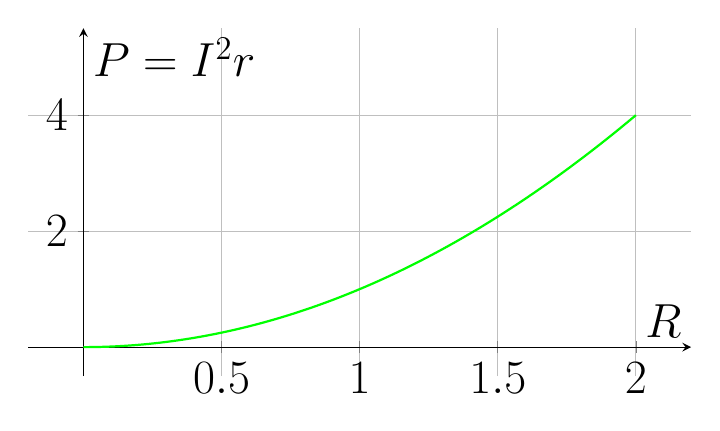
\begin{tikzpicture}
    \begin{axis}[
        width=10cm, height=6cm,
        axis lines=middle,
        xlabel={$R$},
        ylabel={$P = I^2r$},
        xmin=0, xmax=2,
        ymin=0, ymax=5,
        grid=both,
        samples=200,
        domain=0:2,
        enlargelimits,
        legend pos=south east
      ]
    \addplot[green, thick, domain=0:2] {(x*x)*1)}; % E = 4, r = 4 为例
  \end{axis}
\end{tikzpicture}\\
\textbf{电源热功率与外电阻图像}\\
\begin{tikzpicture}
  \begin{axis}[
      width=10cm, height=6cm,
      axis lines=middle,
      xlabel={$R$},
      ylabel={$P = \dfrac{E^2}{(R + r)^2}r$},
      xmin=0, xmax=2,
      ymin=0, ymax=5,
      grid=both,
      samples=200,
      domain=0:6,
      enlargelimits,
      legend pos=south east
    ]
    \addplot[black, thick, domain=0:2] {(4/(x + 1)^2};
    \end{axis}
  \end{tikzpicture}\\
  \textbf{电源输出功率与电流图像}\\
  \begin{tikzpicture}
    \begin{axis}[
        width=10cm, height=6cm,
        axis lines=middle,
        xlabel={$R$},
        ylabel={$P = (\dfrac{E}{r}-I)Ir$},
        xmin=0, xmax=2,
        ymin=0, ymax=1,
        grid=both,
        samples=200,
        domain=0:2,
        enlargelimits,
        legend pos=south east
      ]
      \addplot[blue, thick, domain=0:2] {x*(2-x)};
    \end{axis}
  \end{tikzpicture}\\
  \textbf{电源输出功率与外电阻图像}\\
  \begin{tikzpicture}
    \begin{axis}[
        width=10cm, height=6cm,
        axis lines=middle,
        xlabel={$R$},
        ylabel={$P = \dfrac{E^2}{(R + r)^2}R$},
        xmin=0, xmax=6,
        ymin=0, ymax=1,
        grid=both,
        samples=200,
        domain=0:6,
        enlargelimits,
        legend pos=south east
      ]
      \addplot[red, thick, domain=0:6] {4/(x+1/x+2)};
    \end{axis}
  \end{tikzpicture}\\
}
\noindent\textbf{电源功率图像说明：}
\begin{itemize}
  \item 上面的小于等于的意思是，存在一个极大值
  \item $\frac{E}{r}$为短路电流
  \item 蓝色直线为电源总功率
  \item 绿色抛物线为电源热功率
  \item 红色抛物线为电源输出功率
  \item 电阻线经过了放大，这样能够清晰地看出输出功率随电阻变化先增大后减小，在内阻等于外阻的时候取得极值
\end{itemize}

\noindent\textbf{电功率注意事项：}
\begin{itemize}
  \item 正常工作意味着用电器的全部物理量为额定值
  \item 电动机这样的非纯电阻元器件不能正常工作时，可看作纯电阻
  \item 灯泡虽然会发热，但仍然看成定值电阻
  \item \textbf{不要使用非纯电阻两端电压得到电流或电阻。}$r\neq \frac{U}{I}$
  \item 非纯电阻的内阻也不要与其他电路电阻进行串并联
  \item 通过输出功率最大时电阻情况，此时内外电压相等，大小为$\frac{E}{2}$
  \item 外电阻增大，电源总功率和电源热功率都会减小，电源效率也会升高
  \item 外电压增大，输出功率先增大后减小，当外电压等于$\frac{E}{2}$时，输出功率最大
  \item 此时电源效率为50\%
\end{itemize}

\textbf{电路实验：电表接法选择}

\noindent\textbf{电流表的内外接判断：}
\begin{itemize}
  \item 电流表内接时，因为电流表分压，电阻测量值偏大
  \item 电流表外接时，因为电压表分流，电阻测量值偏小
\end{itemize}

\noindent\textbf{判断电表接法方法一：临界值法}
\begin{itemize}
  \item 如果$R_x<\sqrt{R_VR_A}$，采用外接法
  \item 如果$R_x>\sqrt{R_VR_A}$，采用内接法
\end{itemize}

\noindent\textbf{判断电表接法方法二：试触法}
\begin{itemize}
  \item 如果两次内外接过程中，电流表读数变化较大，即电压表分流明显，采用内接法
  \item 如果电压表读数变化较大，即电流表分压明显，采用外接法
\end{itemize}

\noindent\textbf{判断电表接法方法三：内阻已知法}
\begin{itemize}
  \item 电流表内阻已知，采用内接法
  \item 电流表内阻未知，采用外接法
\end{itemize}

\noindent\textbf{电表量程选择：}
\begin{itemize}
  \item 可以略超量程，但是不能选择过大的量程
  \item 例如电源电压为4V，选择3V的电压表是可行的
  \item 但是选择15V的电压表就不合适了
\end{itemize}

\textbf{电路实验：滑动变阻器选取原则}

按照如下原则依次进行：
\begin{itemize}
  \item 要求大范围，电压或电流从0开始，测量用电器伏安特性曲线，分压式接法
  \item 滑动变阻器总电阻小于用电器，分压式接法
  \item 滑动变阻器总电阻和用电器接近，限流式接法
  \item 需要节省能量，尽可能节约，限流式接法
\end{itemize}

\noindent\textbf{滑动变阻器阻值选择简化版：}
\begin{itemize}
  \item 限流式：$R_{\text{滑动变阻器}}$略大于或约为 $3\sim 5$ 倍 $R_x$
  \item 分压式：$R_{\text{滑动变阻器}}<R_x$（需要电压能从0开始）
\end{itemize}

\noindent\textbf{电路连接示例：}

\noindent\textbf{电流表外接法与滑动变阻器分压式接法：}
\begin{center}
  \begin{circuitikz}[european resistors]
    \tikzstyle{every node}=[font=\LARGE]
    \draw (7.5,16.5) to[battery] (10,16.5);
    \draw (7.5,17.75) to[potentiometer] (12.5,17.75);
    \draw (10,16.5) to[normal open switch] (12.5,16.5);
    \draw (10,18.25) to[short] (10,19);
    \draw (10,19) to[short] (12.5,19);
    \draw (12.5,16.5) to[short] (12.5,17.75);
    \draw (12.5,19) to[short] (12.5,21.5);
    \draw (7.5,21.5) to[rmeter, t=V] (12.5,21.5);
    \draw (7.5,20.25) to[european resistor] (12.5,20.25);
    \draw (7.5,16.5) to[rmeter, t=A] (7.5,21.5);
  \end{circuitikz}
\end{center}

\noindent\textbf{电流表内接法与滑动变阻器限流式接法：}
\begin{center}
  \begin{circuitikz}[european resistors]
    \tikzstyle{every node}=[font=\LARGE]
    \draw (7.5,16.5) to[battery ] (10,16.5);
    \draw (10,16.5) to[normal open switch] (11.25,16.5);
    \draw (11.25,16.5) to[potentiometer] (13.75,16.5);
    \draw (7.5,17.75) to[european resistor] (10,17.75);
    \draw (10,17.75) to[rmeter, t=A] (12.5,17.75);
    \draw (7.5,19) to[rmeter, t=V] (12.5,19);
    \draw (7.5,16.5) to[short] (7.5,19);
    \draw (12.5,17) to[short] (12.5,17.75);
    \draw (12.5,17.75) to[short] (12.5,19);
  \end{circuitikz}
\end{center}

\textbf{电路实验：半偏法测电阻}

\noindent\textbf{半偏法测电阻一定有误差}

\noindent\textbf{限流式电路中的半偏法：}
\begin{itemize}
  \item 半偏法假定干路电流不变
  \item 但先满偏后半偏时，干路电流将会变大
  \item 另一条未确定电流的支路电流将会比计算值偏大
\end{itemize}

\noindent\textbf{结论：限流式，半偏法测量值偏小；分压式，半偏法测量值偏大}

\noindent\textbf{电桥测电阻所需设备：}
\begin{itemize}
  \item 高精度电流计（可以左右偏转，量程越小越好，精度越大越好）
  \item 两个已知阻值的定值电阻（或者使用均匀的电阻丝，通过长度比值得到电阻之比）
  \item 一个电阻箱
\end{itemize}

\subsection{磁场}

\begin{formulatab}{磁场}
  \multicolumn{2}{l}{\textbf{磁场强度与力}}\\
  磁场强度&$B=\frac{F}{Il}$\\
  安培力&$F=Il\times B=BIl\sin\theta$\\
  洛伦兹力&$F=qv\times B=qvB\sin\theta$\\
  \multicolumn{2}{l}{\textbf{带电粒子的运动}}\\
  洛伦兹力做向心力&$qvB=m\frac{v^2}{R}=m\omega^2R=mv\omega$\\
  半径&$R=\frac{mv}{qB}$\\
  周期&$T=\frac{2\pi m}{qB}$\\
  角速度&$\omega=\frac{qB}{m}$\\
  运动时间&$t=\frac{\theta m}{qB}=\frac{\theta R}{v}$\\
  加速电场进入磁场半径&$R=\frac1B\sqrt{\frac{2mU}{q}}$\\
  \multicolumn{2}{l}{\textbf{电磁应用}}\\
  速度选择器&$qE=qvB$\\
  质谱仪&$R=\frac1B\sqrt{\frac{2mU}{q}}$\\
  霍尔电压&$U=\frac1{nq}\frac{IB}{d}$\\
  \multicolumn{2}{l}{\textbf{回旋加速器}}\\
  最大速度&$v_{max}=\frac{qBR}{m}$\\
  最大动能&$E_{kmax}=\frac{q^2B^2R^2}{2m}$\\
  电场周期&$T=\frac{2\pi m}{qB}$\\
  加速次数&$n=\frac{qB^2R^2}{2mU}$\\
  加速总时间&$t=\frac{\pi BR^2}{2U}$\\
\end{formulatab}

\noindent\textbf{磁场力注意事项：}
\begin{itemize}
  \item 地磁场水平方向上从南指向北
  \item 竖直方向北半球有向下的分量，南半球有向上的分量
  \item 磁场是真实存在的特殊物质，磁感线是人为创造的模型
  \item 磁感线在磁体外部从N极指向S极，在磁体内部从S极指向N极
  \item 小磁针N极受力方向为磁场方向
  \item 安培定则：右手握住导线，大拇指指向电流方向，此时四指环绕方向为磁场方向
  \item 右手螺旋定则：右手握住螺线管，四指环绕方向为电流方向，大拇指指向磁体内部磁场方向
  \item 同向电流导线相互吸引，反向电流导线相互排斥
  \item 左手定则：四指伸直指向电流方向，磁感线穿过掌心，大拇指指向安培力方向
  \item 安培力方向与电流方向和磁场方向都垂直，电流方向和磁场方向垂直时安培力最大
  \item 左手定则中四指指向正电荷移动方向与负电荷移动反方向
  \item 洛伦兹力方向与速度方向和磁场方向都垂直，速度方向和磁场方向垂直时洛伦兹力最大
  \item 洛伦兹力不能影响电荷的速度大小，只能改变电荷的运动方向
  \item 洛伦兹力可以通过影响正压力的方式影响滑动摩擦力，进而影响速度
  \item 沿电流方向速度引起的洛伦兹力分力是安培力的微观本质
  \item 洛伦兹力分力可以做功，影响物体的能量分配
\end{itemize}

\noindent\textbf{电磁应用注意事项：}
\begin{itemize}
  \item 速度选择器提高精度可以增加板长、减小板间距
  \item 速度选择器只能从一个方向进入
  \item 速度选择器无法分辨电性
  \item 质谱仪根据不同的比荷得到不同的半径
  \item 质谱仪中比荷越大半径越小；比荷越小半径越大
  \item 霍尔电压中，载流子的电性直接影响电压的正负极
  \item 回旋加速器中，电场加速时间忽略不计
  \item 回旋加速器加速总时间和粒子的比荷无关
  \item 回旋加速器加速不同比荷的粒子需要调整电压频率
\end{itemize}

\noindent\textbf{带电粒子运动注意事项：}
\begin{itemize}
  \item 直线性边界下，进入夹角等于离开夹角，速度偏转角为$2\theta$
  \item 速度偏转角就是圆周运动的圆心角
  \item 两个对称进入磁场的粒子，从同一点对称离开磁场
  \item 圆形磁场沿半径进入磁场，沿半径离开磁场
  \item 平抛运动中，离开极板区域的最小速度为$v_0=\sqrt{al}$，并且此时夹角为$45^{\circ}$
\end{itemize}

\subsection{电磁感应}

\begin{formulatab}{电磁感应}
  感应电动势定义&$E=\frac{W}{q}$\\
  法拉第电磁感应定律&$E=n\left|\frac{\Delta\Phi}{\Delta t}\right|$\\
  闭合回路欧姆定律&$I=\frac{E}{R+r}$\\
  导体棒切割磁感线&$E=Blv$\\
  回路电荷量&$q=\frac{n\Delta\Phi}{R+r}$\\
  感应电流功率&$P=EI=I^2(R+r)$\\
\end{formulatab}

\textbf{楞次定律}

感应电流（或感应电动势）的方向总是阻碍引起感应电流的磁通量变化。判断方向时可先判断原磁通量如何变化，再确定“阻碍变化”的磁场方向，最后用右手定则判断感应电流方向。

\textbf{电磁感应定律}

法拉第定律定量给出感应电动势大小，楞次定律定性给出方向。解题时通常先由磁通量变化求$E$，再结合闭合电路欧姆定律求$I$，最后再求力、功率和能量转化关系。

\textbf{电动机模型}

电动机模型通常与安培力和能量转化结合：导体在磁场中受力转动，电能转化为机械能并伴随焦耳热。分析时可结合$P=UI$、$P_{\text{热}}=I^2R$与输出功率关系。

\textbf{单棒模型}

单导体棒切割磁感线时，常用$E=Blv$建立电动势，再由回路总电阻求电流。若含外力做功，常结合动能定理或功能关系分析速度变化与最终稳定状态。
\textbf{电阻模型}
最简单的模型，构成单回路，回路中电阻可以进行合并，使得只有一个总电阻，注意问题中电阻是否可变，以前出题可能会让导轨具有电阻，会随着位移增加均匀增大或者减小。
该模型一般有初速度或者外力，外力研究一般让其不变，如果是可变外力，那么很有可能是与安培力相等的，或者让单棒能够匀变速运动的外力。结合题目调整外力的表达式即可，研究我们以恒定外力为例。
接着以同时具有初速度与恒力的单棒为例进行分析，其中初速度的方向与外力的方向是指向电阻还是背对电阻不影响，（固定电阻的情况下）。那么问题可以首先分成两类，初速度方向与外力方向一致与不一致。
这两种情况有一点是相同的，安培力一定时刻与速度方向相反，这很容易通过楞次定律判断。接着第一种一致的情况，需要判断安培力的大小与外力的大小关系，如果安培力大于外力，那么单棒做减速运动，直到安培力等于外力，单棒做匀速运动。
列出单棒的牛顿运动定律、动能定理、动量定理。首先是牛顿运动定律：如果外力大于安培力，$F-F_{\text{安}}=ma$，接着是动能定理：$Fx-F_{\text{安}}x=\frac{1}{2}mv^2-\frac{1}{2}mv_0^2$，最后是动量定理：$Ft-F_{\text{安}}t=mv-mv_0$。其中安培力做功无法直接求出，但是在这种情况下，安培力一定做负功，并且就是回路中产生的焦耳热。在动量定理中，安培力的冲量有两种表达式，也就是$I_{\text{安}}=BLq=\frac{B^2L^2x}{R}$。
如果外力小于安培力，$F_{\text{安}}-F=ma$，接着是动能定理：$F_{\text{安}}x-Fx=\frac{1}{2}mv^2-\frac{1}{2}mv_0^2$，最后是动量定理：$F_{\text{安}}t-Ft=mv-mv_0$。和前面类似注意一下大小关系即可。
如果安培力小于外力，那么单棒做加速运动，直到安培力等于外力，单棒做匀速运动。两者的最终匀速速度可以直接得到，$v=\frac{F}{B^2L^2}R$。在反向之后可以看成初速度为0的，公式和前面的一样，关注一下减速到0这个过程。此时牛顿运动定律是$F+F_{\text{安}}=ma$，动能定理是$F_{\text{安}}x+Fx=\frac{1}{2}mv^2$，动量定理是$F_{\text{安}}t+Ft=mv$。注意一下大小关系即可。

第二种情况，外力与初速度方向相反与安培力方向相同，那么单棒做减速运动，一直到速度为0，然后开始反向加速，直到安培力等于外力，单棒做匀速运动。两者的最终匀速速度可以直接得到，$v=\frac{F}{B^2L^2}R$。
最终你会发现，只要有外力，单棒最终都会做匀速运动，并且匀速速度为$v=\frac{F}{B^2L^2}R$。那反之，如果外力为0，那么单棒最终都会停下来。

\textbf{电源模型}
电源模型相对复杂得多，原因很简单，电源会施加一个额外的电流，使得不能直接通过运动方向得出安培力与速度反向。
单棒可能有初速度可能没有，可能有外力可能没有。下面研究的时候以全都存在作为例子。
先进行问题的分类讨论，首先是初速度方向产生的感应电动势可能与电源的相同或者相反，外力可能与电源产生的电流对应的安培力方向相同或者相反，这样就是四种情况。我们后面可以发现其实四个过程中存在一个先后发生而非并列的关系，类似于前面电阻模型中的先减速后加速过程。那最初研究我们就不做这样的前瞻性判断，直接分成四种不同的情况去研究。
第一种情况，初速度产生的感应电动势与电源的电动势相叠加，也就是正极与负极相连接。并且外力与电源产生的电流对应的安培力方向相同。此时初速度产生的安培力与初速度方向相反，也就与外力方向相同。此时单棒会减速运动，减速后安培力减小，但是外力仍然存在则并不会匀速，而是一直减小到0，接着外力和电源提供的安培力会使得单棒反向加速，而感应电动势此时因为速度反向而与电源的电动势抵消，单棒的加速度在逐渐减小，等到两个电动势相等时，单棒的安培力等于0，单棒此时只收到外力，继续加速。感应电动势进一步增大，大于电源电动势，安培力也开始反向增大，逐渐增大到与外力相等时，单棒做匀速运动。最终速度可以求出：$F=\frac{BL(BLv-E)}{R}$。进一步求出速度即可。所以你会发现$E=BLv$是一个特殊值，但并不是匀速运动的那个条件，因为外力存在导致的，如果此类问题没有外力，那么匀速运动的条件就是$E=BLv$。
第二种情况，初速度产生的感应电动势与电源的电动势相叠加，也就是正极与负极相连接。并且外力与电源产生的电流对应的安培力方向相反。此时外力一开始就与合成的安培力相反，单棒具体运动状态需要观察一下安培力的大小关系，如果安培力大于外力，那么单棒做减速运动，而减速的安培力随着速度的减小在减小，有可能外力直到速度等于0也没有大于等于安培力，也就是条件：$F\leq \frac{BLE}{R}$。这样单棒一定会减速到0，然后反向运动。还有可能减小并且外力比电源提供的安培力大一点，所以以另一种形式匀速：$F=\frac{BL(BLv+E)}{R}$。另一种即是外力较大($F>\frac{BL(BLv_0+E)}{R}$)，单棒做的是加速运动，加速直到安培力等于外力，单棒做匀速运动。最终速度可以求出：$F=\frac{BL(BLv+E)}{R}$。进一步求出速度即可。
\textbf{电容器模型}

\textbf{双棒模型}

双棒模型关注两棒速度关系、回路电流方向和系统能量分配。常见处理方法是先由相对运动确定感应电动势，再联立受力与运动方程，最后结合能量守恒或动量关系求解。
